\documentclass[a4paper,12pt]{article}

\usepackage[utf8]{inputenc}
\usepackage{polski}
\usepackage{a4wide}

\usepackage[colorlinks=true,linkcolor=blue,urlcolor=blue]{hyperref}

\usepackage[pdftex]{graphicx}



\usepackage{microtype}

\hypersetup{
	unicode = true,
	pdfauthor = {},
}

\title{Cumulonimbus}
\author{}

\begin{document}
\maketitle

\section{Wstęp}

Projekt Cumulonimbus ma na celu stworzenie systemu plików opartego na chmurze. Chmurę stanowi Swift stanowiący część intensywnie rozwijanego projektu OpenStack. Swift zapewnia funkcjonalność potrzebna do przechowywania i zrządzania danymi w chmurze. 

Od strony klienta montującego nasz system plików wykorzystujemy FUSE. Czyli moduł jądra który pozwala w prosty sposób zaimplementować funkcjonalność systemu plików. 

Projekt złożony jest z trzech komponentów, stanowiących odseparowane warstwy. Są nimi cfuse, fs, cloud.

\section{Jak to działa}
\begin{figure}[htb]
\begin{center}
\leavevmode
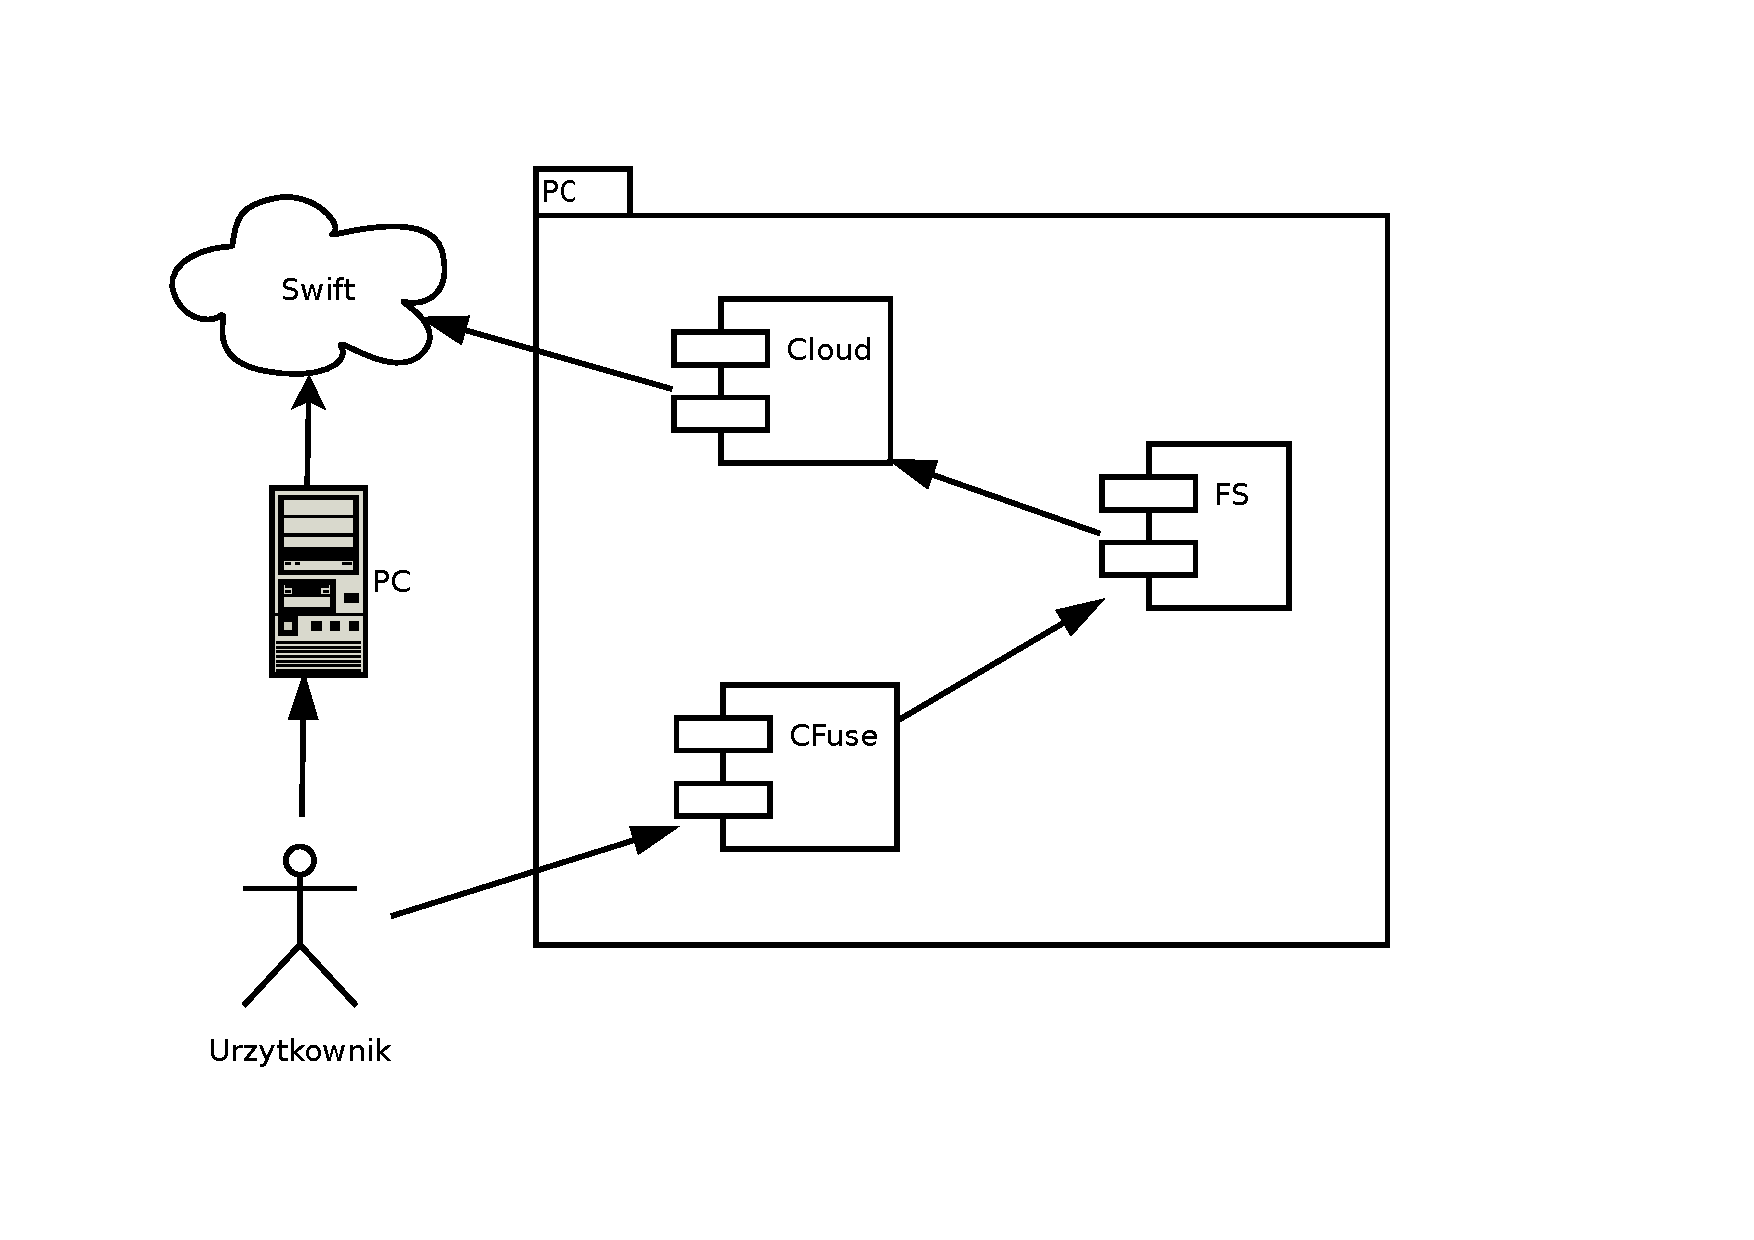
\includegraphics[width=\textwidth]{arch_komunikacja2.pdf}
\end{center}
\caption{Struktura Cumulonimbusa}
\label{fig:dia_arch_komunikacja}
\end{figure}

\subsection{Montowanie}

Podczas montowania następuje zalogowanie użytkownika do zadanej instancji Swift oraz ustanowienie sesji. Modułem do którego odwołuje się użytkownik jest cfuse. Podczas tworzenia obiektu cloud.Swift następuje zestawienie połączenia i token sesji wraz z utworzonym obiektem zostają przekazane w konstruktorze do klasy FS. 

Po udanym zamontowaniu systemu plików Cumulonibus, uproszczony schemat klas został zaprezentowany na rysunku \ref{fig:dia_arch_klasy}.

\begin{figure}[htb]
\begin{center}
\leavevmode
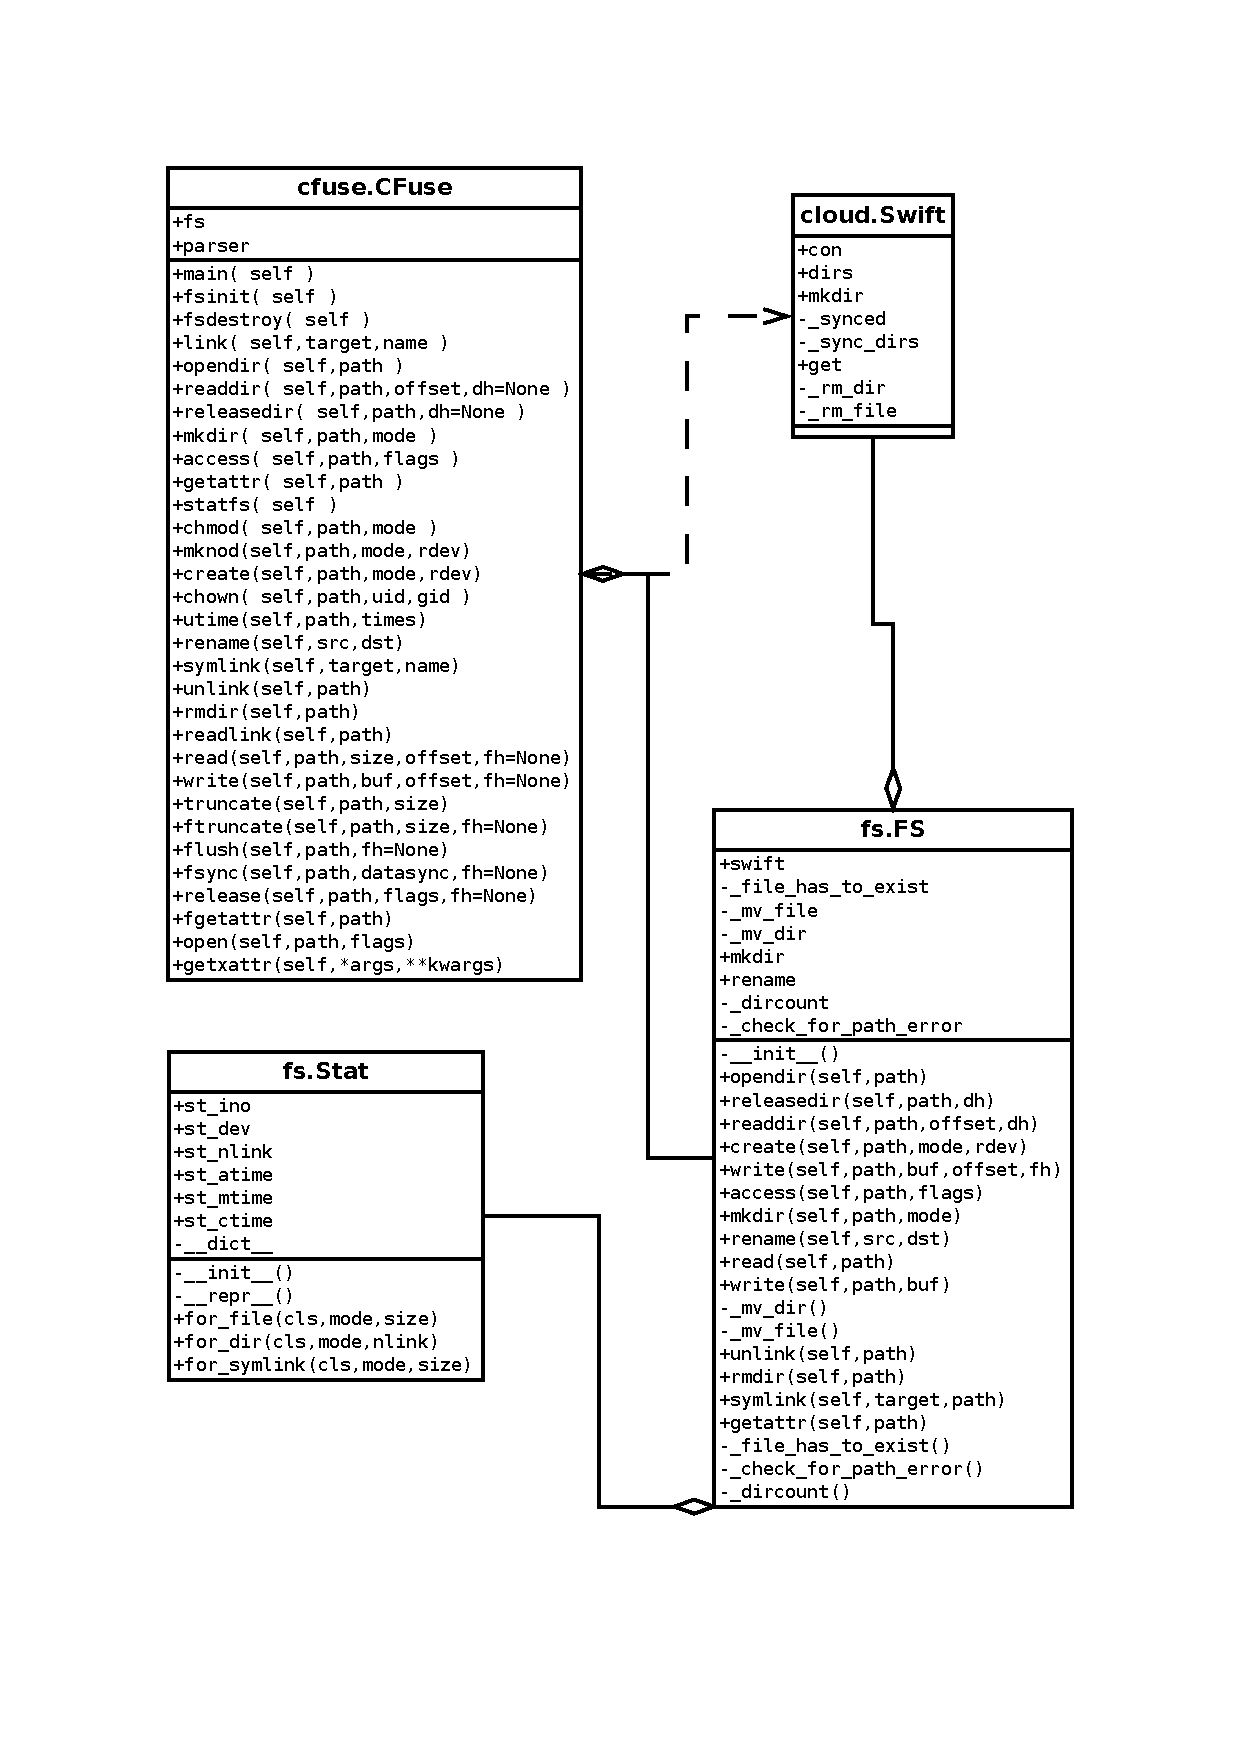
\includegraphics[width=\textwidth]{arch_klasy.pdf}
\end{center}
\caption{Diagram klas po zamontowaniu}
\label{fig:dia_arch_klasy}
\end{figure}


\subsection{Praca z Cumulonibus'em}

Wszystkie operacje utworzenia, skasowanie, przeniesienia...itp. wykonane nad zamontowanym drzewem katalogów są przechwytywane przez moduł FUSE'a. Z kolei te wywołania są przekazywane do obiektu klasy CFuse która podczas montowania rejestruje obsługę tego poddrzewa.

Obiekt CFuse, stanowi jedynie warstwę mapująca wywołania API FUSE'a w celu uniezależnienia się od jego implementacji. Faktyczna logika zarządzająca systemem plików jest obiekt klasy FS. Warstwa fs komunikuje się również pośrednio z faktyczną chmurą za pomocą modułu cloud. 

Warstwa cloud mapuje wywołania API Swift'a. 


\end{document}
